\section{IRR-Filters}
\subsection{Design of IRR-filters}
Design of IRR-filters is done in the following steps:
\begin{enumerate}
  \item The specifications of the IRR-filter.
  \item The transfer function of the IRR-filter.
  \item The optimal realization of the IRR-filter.
  \item Program for signalprocessing or a circuit diagram for analog
    signalprocessing.
\end{enumerate}
\subsection{Matched z-transform}
By using the matched z-transform, the poles and zeros of the IRR-filter are directly transferred to the z-plane. The transfer function of the IRR-filter is given by:
$$z=e^{sT}$$
\subsubsection{1. Order IRR-filters}
The transfer function for a first order system is given by:
$$H(s)={\frac{s+A_{0}}{s+B_{0}}}={\frac{s-\sigma_{1}}{s-\sigma_{2}}}$$
where $-A_{0}=\sigma_1$ is a real zero and $-B_{0}=\sigma_2$ is a real pole of the IRR-filter.

A digital first order transfer function is given by:
$$H(z)={\frac{z-e^{\sigma_1 T}}{z-e^{\sigma_2 T}}}=\frac{1-e^{\sigma_1 T}z^{-1}}{1-e^{\sigma_2 T}z^{-1}}$$

A first order system without a zero is given by:
$$H(s)=\frac{\omega_a}{s+\omega_a}$$
Using the matched z-transform, the digital transfer function is given by:
$$H(z)=\frac{1}{1-e^{\sigma_1 T}z^{-1}}$$
where $\sigma_1$ is the pole of $H(s)$ and $T$ is the sampling period.\\
The transfer function $H(z)$ does not have a DC-gain of 1. To get a DC-gain of 1, the transfer function is multiplied by a gain factor $a_0$:
$$H(z)=\frac{a_0}{1+b_1z^{-1}}$$
where $b_0=-e^{\sigma_1 T}$ and $a_0=1+b_1$.\\
The corresponding digital realization structure:
\begin{center}
  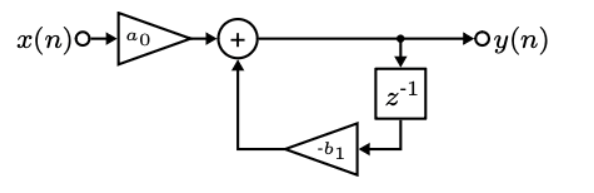
\includegraphics[width=0.5\textwidth]{Images/Matched-z-1th.png}
\end{center}
\subsubsection{2. Order IRR-filters}
The transfer function for a second order system with complex conjugate pole and zero pair is given by:
$$H(s)={\frac{s^{2}+A_{1}s+A_{0}}{s^{2}+B_{1}s+B_{0}}}$$
which has zeros in $s_1=\sigma_1+j\omega_1,s_1^*=\sigma_1-j\omega_1$ and poles in $s_2=\sigma_2+j\omega_2,s_2^*=\sigma_2-j\omega_2$

Using the matched z-transform:
$$H(z)={\frac{(z-e^{\sigma_{1}T}e^{j\omega_{1}T})(z-e^{\sigma_{2}T}e^{-j\omega_{1}T})}{(z-e^{\sigma_{2}T}e^{j\omega_{2}T})(z-e^{\sigma_{2}T}e^{-j\omega_{2}T})}}$$
\subsection{Impulse invariance method}

\subsection{Examples}
\subsubsection{Example 1: Matched 1. order z-transform}
Consider the following analog first order lowpass filter with cutoff frequency $\omega_a=2\pi f_a$ where $f_a=\SI{300}{\hertz}$:
$$H(s)=\frac{\omega_a}{s+\omega_a}=\frac{1885}{s+1885}$$
which has a pole in $s_1=\sigma_1=-1885$.\\
Find the digital IRR-filter using the matched z-transform with sampling frequency $f_s=\SI{16}{\kilo\hertz}$.

\noindent\rule{\textwidth}{1pt}

The coefficients of the digital IRR-filter are given by:
$$b_1=-e^{\sigma_1 T}=-e^{-1885\cdot\frac{1}{16000}}=-0.8889$$
$$a_0=1+b_1=0.1111$$
The digital lowpass filter is given by:
$$H(z)=\frac{a_1}{1+b_0z^{-1}}=\frac{0.1111}{1-0.8888z^{-1}}$$
